\documentclass[12pt]{IEEEtran}

\usepackage[english]{babel}
\usepackage[utf8x]{inputenc}
\usepackage{amsmath}
\usepackage{graphicx}

\title{Requirements and Specifications}
\author{Bryan Ceberio-Lucas, \and Ethan Eldridge, \and Peter LeBlanc, \and Phelan Vendeville }

\begin{document}
\maketitle

\begin{abstract}
	This document contains the specifications of CS 205 Software  Engineering's final project, an implementation of Rat-a-tat Cat. These standards and requirements will be followed by all team members. The following terms and descriptions must be clear to all members so that the system is a cohesive and comprehendable system.
\end{abstract}

\tableofcontents

\section{Terms and Definitions}
\label{sec:TermsDefinitions}
	\begin{description}
		\item[Must] If a specification uses the word Must, it is mandatory that all team members follow this requirement. E.g.  \textit{The System \textbf{must} handle all possible URLs and direct the user's to an appropriate page.} 
		\item[Shall] If a specification uses the word Shall, then the System must respond to the specification in the detailed way. E.g. \textit{The system \textbf{shall} perform operations in a timely manner and no operation will take more than 10 seconds}
		\item[Gantt] A bar graph used to visualize a project schedule
		\item[Glow] To glow is to surround an object with a faint highlight that indicates that the User may interact with this object.
		\item[State] The System's internal state is kept using a Stack of strings that indicate the current and next state of the System, this collection is refered to as the State and can be pushed, popped, and 	peeked.
		\item[Magic Numbers] \hspace{4em} Hard-coded numerical constants 
		\item[Knock] \hspace{.5em} The button press that determines a round is over and the cards should be overturned when gameplay returns to the user who knocked.
		\item[Light-Box] \hspace{2em}An overlayed $<div>$ tag containing the contents of a webpage, usually placed above the current page.
		\item[REST] Representational state transfer, this is the primary method of resource sharing between clients and servers within the world wide web. It emphasizes a stateless environment, which can cause difficulties when designing game systems and web-pages that require a large amount of Client Server interaction.
	\end{description}


\section{Introduction}
\label{sec:introduction}

	Rat-a-Tat-Cat is an award winning children’s card game produced by Gamewright. Using a set of easy to learn and intuitive rules, Rat-a-Tat-Cat teaches memory, simple math, and probability skills to players over the course of the game. 
	
	It is our goal to create a software implementation of this game based on the desires of our client Jason Hibbeler, and falling within the basic constraints of the standard game rules. This implementation will be a web-based, interactive and graphical representation of Rat-a-Tat-Cat, providing the user with an experience equal to or exceeding that of the physical game.

\section{Scope and Purpose}
\label{sec:scope}

\subsection{Scope}
\label{subsec:scope}

	High level scope for this game includes a set of several features to be delivered over the course of several weeks in the University of Vermont Spring Semester. This software product and its features is restricted to academic use and is not to be shipped for profit. The receipt of these features will indicate a fulfillment of obligation on the part of the software engineering team to the client. These high level deliverables include this technical specifications document, comprehensive product testing data documents, and a completed, playable game of Rat-a-Tat-Cat based on the constraints provided by the client.

\subsection{Purpose}
\label{subsec:purpose}

	This document will be used to delineate the behavior, structure and requirements of the Rat-a-Tat-Cat game system, including both functional and nonfunctional elements. This document has been written to be read, and as such will serve as a guide to both developers and the client. It shall provide a followable rubric to the software engineering team for enumeration of executable and deliverable expectations, and give the client a set of expectations to be fulfilled. 
	
	We shall begin the specifications document with an exploration of the project’s functional requirements, then continue with its nonfunctional stipulations. We will outline a series of test cases to ascertain the completion of such exigencies, and conclude with a brief summary of the document.

\section{Rules}
\label{sec:rules}

	The objective of the game is to have the lowest score at the end of the game. Each player is delt 4 cards, facedown at the beginning of the game. Once all players have cards, they are allowed to view the two outermost cards for a short time. From this point on, a player may not look at their cards unless they have a peek power card. 

	Each turn begins with a player making the choice to draw from the discard pile or the deck. If the player draws the top card of the discard pile (which is face up), then they may replace one of their 4 cards with the drawn card. The players turn is now over. However, if a player draws from the deck, depending on the type of card they receive a different action may occur. If the user draws a numeric card, they are able to swap any of their 4 cards with the drawn card. After doing so, whichever card is not used is discarded face up. If the user draws a power card they execute that power. The power card actions are described in detail in \S\ref{subsec:gameplay}. 

	When a player thinks that they have the lowest score and can win the round, they knock on the table and each player is allowed one more turn. After these turns are taken, the players flip their cards over and total their card values. Any power cards in the turned over cards  must be swapped with the top card of the draw pile. Whichever player has the lowest score wins the round. If a player has accumulated over 60 points they lose or if the draw pile is used up, the game is also over.

\section{Functional Requirements}
\label{sec:funcReq}
	The functional requirements of this project are specified by the Coding Standards in \S \ref{subsec:coding}, Version 			Control standards in \S \ref{subsec:git}, directory and game Architecture in \S 	\ref{subsec:arch}, Artificial Intelligence 		logical overview in \S \ref{subsec:ai}, and Database Design images and naming conventions in \S\ref{subsec:dbdesign}.


\subsection{Coding Standards}
\label{subsec:coding}

	The following standards must be followed by all team members. By defining these standards all code will be readable for 		all members, and no discrepencies between conventions will occur. Each team member is responsible for keeping to these 	standards, and submission of code not keeping to these standards will come under review and the format shall be 			adjusted accordingly. 

	\bfseries Naming conventions \mdseries

	\begin{itemize}
		\item Variable names must be camelcase, descriptive, and self documenting
		\item Class names must begin with a capital letter and use camelcase 
		\item Database table names must begin with a capital letter and use camelcase
		\item Database table names should be short, one word where ever possible
		\item Database field names must be camelcase, beginning with a lowercase letter except for foreign keys
		\item Foreign key fields are prefixed by the foreign tables name, and therefore begin with uppercase letters
		\item Directories must be lowercase and without spaces
		\item File names must be lowercase and without spaces
		\item File names for card images must be the value of the card, or 10-12 for power cards.
		\item All images should end in .png and be of that format
		\item CSS class names must be self-documenting
		\item CSS class names must be camel case
		\item Constants in any form must be all uppercase with underscores between natural breaks
		\item Git tagging must follow the convention of version\_x.y, x must be the major release number, y the minor 					release number
		\item The team leaders repository should be refered to as mainline during remote declaration
	\end{itemize}

	\bfseries Commenting Conventions \mdseries

	At the beginning of each function or class there must be a comment section within triple qoutes defining the following:
	\begin{itemize}
		\item Description of function or class
		\item A list of parameters and types of each
		\item A brief description of the return type of the function
	\end{itemize}

	At the top of each code file there must be a comment section with the following information:
	\begin{itemize}
		\item A description of the file's purpose and intent
		\item A list of the functions or classes defined within the file
		\item The date the file was made
		\item The date of the most recent revision
		\item A list of authors or modifiers of the file. 
	\end{itemize}

	Within HTML each ending $<div>$ should have a comment indicating the id of the opening tag. CSS comments should be 	used to partition style sheet files into managable and well ordered blocks of style. It must be easy to determine which 			content is affected by the style by simpling reading through the comments.

	\bfseries General Conventions and Guidelines  \mdseries

	\begin{itemize}
		\item Conditional statements that involve more than a single variable must use parenthesis
		\item All sensitive information should be passed through posting whenever possible
		\item HTML/CSS should pass validation tests and be well formed and self documenting
		\item Global Variables should only be used when neccesary
		\item Magic Numbers should be avoided whenever possible 
		\item Formal specifications should be made available using the shared Google Drive or through the mainline Git repository
	\end{itemize}

\subsection{Version Control}
\label{subsec:git}

	The version control used to maintain the source code for this System is Git. The following standards must be followed by all team members in order to maintain proper source code management.
	\begin{itemize}
		\item Git commits must be descriptive and verbose
		\item When merging feature and component branches to dev or mainline the option --no-ff must be used
		\item The Git tagging system must be used to maintain stable release checkpoints
		\item The master branch of the mainline repository must be functional
		\item Rebasing commit history is forbidden if the history has been pushed to a remote repository
		\item A team member resolving merge conflicts must ensure the merge is agreeable to both their and the incoming code
		\item All members must have their global config setup with email and name for source code tracking purposes
	\end{itemize}
	

\subsection{Architecture and Structure}
\label{subsec:arch}

	The System shall use the Google App Engine (GAE) and Jinja templating systems to function. The model-view-controller 			paradigm will be implemented, in this instance the model will be the database backend from GAE. The view will be 				comprised of Jinja templates, Javascript/JQuery, and CSS. The python files used by the GAE will handle all control 			information and dictate the flow control of the System. The project must be organized, and the directory structure will 			be as follows:
	
	%Dont want the list to be split accross pages
	\newpage

	\begin{itemize}
		\item \texttt{python/}
		\item \texttt{config/}
		\item \texttt{templates/}
		\item \texttt{css/}
		\item \texttt{scripts/}
		\item \texttt{images/}
		\item \texttt{userimages/}
		\item \texttt{sounds/}
	\end{itemize}

	These directory names are self explanatory besides the difference between \texttt{images} and \texttt{userimages}. 			The \texttt{userimages} directory is a location where user uploaded images may be stored, this directory is kept 				separate for security purposes. 

	Each URL handled by the GAE framework and our configuration files is mapped to a python controller in a many to one 			relationship. The URL to python controller mapping is defined as follows:
	
	\begin{center}
		\begin{tabular}{| c | c |}\hline
			\multicolumn{1}{|c}{URL} & \multicolumn{1}{c|}{ Handler Name }\\\hline
			 \texttt{/}			& MasterControlProgram\\\hline
			 \texttt{/scores} 		& ScoresHandler\\\hline
			 \texttt{/game} 		& GameHandler\\\hline
			 \texttt{/playerinfo}	& PlayerInfoHandler\\\hline
			 \texttt{/characterchoice} & CharacterHandler\\\hline
			 \texttt{/difficulty}		& DifficultyHandler\\\hline
		\end{tabular}
	\end{center}

\subsection{Artificial Intelligence}
\label{subsec:ai}

	The artificial intelligence (AI) within the System is stochastic in nature. A difficulty modifier passed via the games start up 	parameters influences the reliability of the AI's memory via a decay rate. Each level of difficulty effects the decay rate 			of the memory as well as the baseline of remembrance. The AI is not all knowing, and keeps estimates of both its and 			the opponents cards. Using these estimates a strategy can 	be used to determine when to knock and when to use 			power cards. For each of the four cards in the AI's hand a rate of memory decay is kept. This value determines how well 	the AI remembers the value of the card and is decremented each round according to the decay rate value 				stored within the AI.

	\begin{description}
		\item[Swap Strategy] \hspace{3em} Using an internal estimate, the AI selects it's highest known card and 						switches it with the players lowest known card. The AI can determine what the players cards are based on 				if the Player has drawn from the discard pile or swapped with one of the AI's known cards. In the case of 					no cards being known -- whether in selection of its own highest card or the users -- a random card is 					chose. 
		\item[Peek Strategy] \hspace{3em} The AI will always select a card it does not know to peek. If all the values are 			known, the AI will select the card with the lowest decayed value, and that value will be reset to 1.
		\item[Knocking] \hspace{3em}  The AI will knock when it has reasonable confidence that its internal estimate of its 			own score is higher than the players.
	\end{description}

	The AI will also keep track of internal statistics to send to the database later. This is primarily a logging function and is an 	optional part of the AI implementation.

\subsection{Database Design}
\label{subsec:dbdesign}

	The database backend is composed of two tables: \texttt{Players} and \texttt{Games}. The field names are shown in 			figure \ref{fig:dbschema}, you can see by the figure that the \texttt{Games} table uses a foreign key referencing the 			playerID within the \texttt{Players} table. This serves to link a user to their scores and allows for the creation of 				leader-boards and other statistics that encourages competition and replay value.
	
	\begin{figure}[ht]
		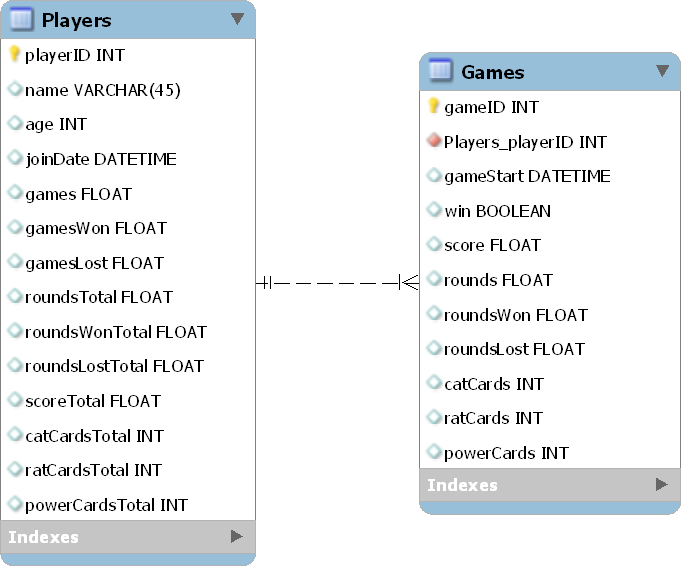
\includegraphics[width=0.5\textwidth]{DatabaseDiagram.png}
		\caption[Database table design]{ Database Schema of the Players and Games tables.}
		\label{fig:dbschema}
	\end{figure}

	The querying of the database during gameplay is shown in figure \ref{fig:dbflow}. The System shall have failsafe 			methods in place so that no in-progress games or games that are terminated unexpectedly affect the statistics for each 		player. A players name and age are the only user supplied information that is entered into the database. The other 			fields are computed by execution and completion of the game.

	\begin{figure}[b]	
		\centering
		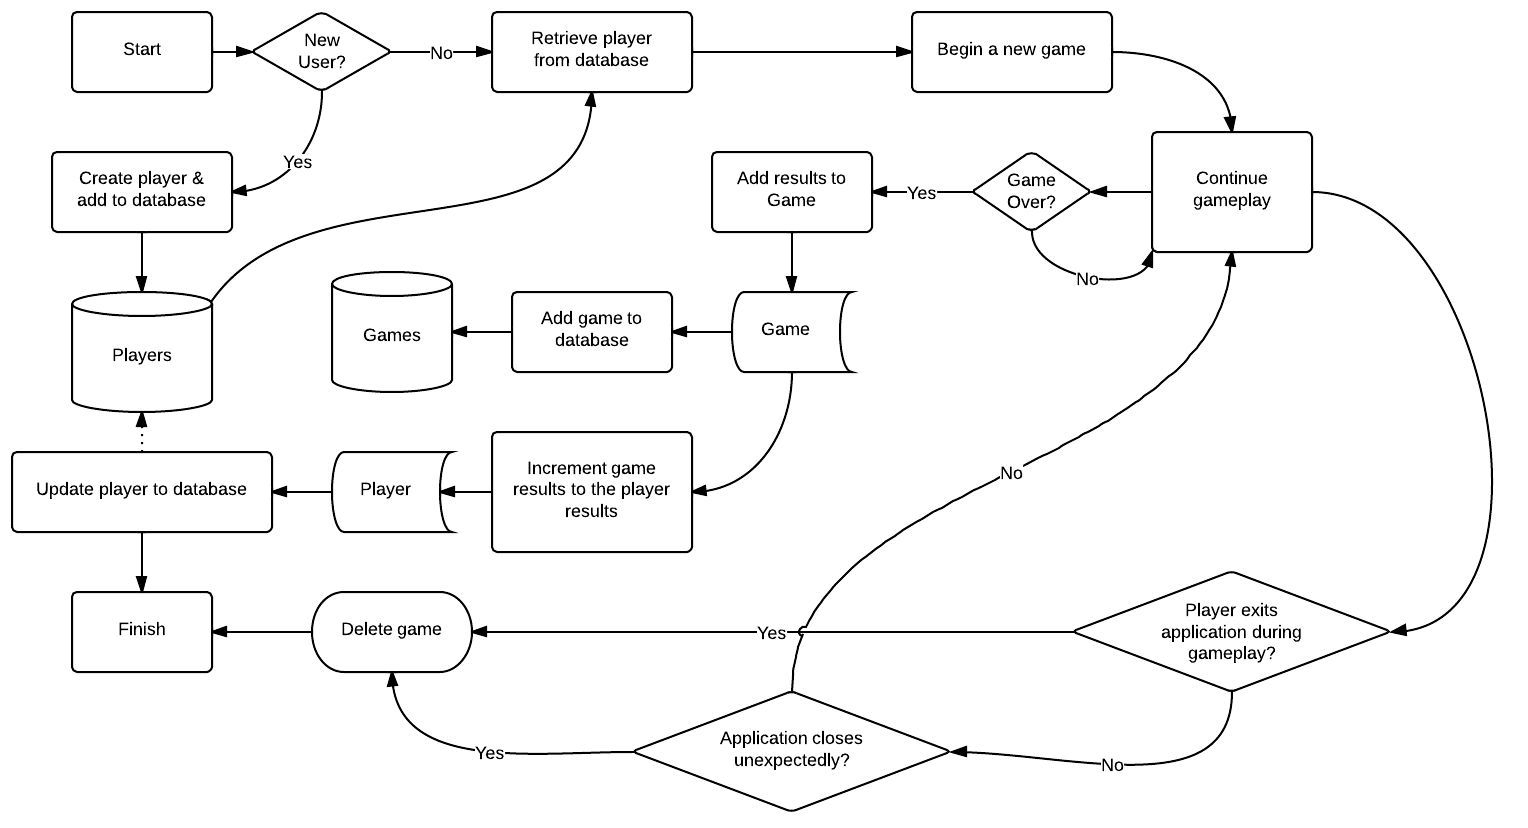
\includegraphics[width=0.5\textwidth]{DatabaseFlowChart.png}
		\caption[Database Query Flow]{ The overall timing and triggers of database interactions from within the game.  }
		\label{fig:dbflow}
	\end{figure}


\section{Non-Functional Requirements}
\label{sec:nonFuncReq}

\subsection{User Interface}
\label{subsec:ui}
	The user interface shall be constructed so as to be intuitive and easy to use. A player communicating with the interface should need little to no instruction in order to execute decisions and allow the gameplay to flow. Although the interface does not teach the actual mechanics of gameplay, it should be structured in such a way as to funnel the user into gameplay decisions with a minimal amount of instruction. 
	
	Ease of use must be measured through usability testing. A series of users will be presented with the interface and supervised using it, with limited contact between the test administrators. The administrators must record their observations and make note of information bottlenecks and constriction points, areas where the flow of the gameplay may become stymied and indicate a change in design is potentially necessary. 
	
	There will be several different interfaces presented to the user, each with a different purpose. The details and design of these interfaces will be examined in the following section. 
	
	\begin{description}
	\item[\textbf{Landing Page:}] \hspace{4em} The landing page will be the first interaction between the user and the game. As such, it must present a clean and polished first impression. The main content area will contain a large splash image presenting introductory art for the game, as well as a series of buttons underneath the splash image.
	
	\begin{figure}[h]
		\centering
		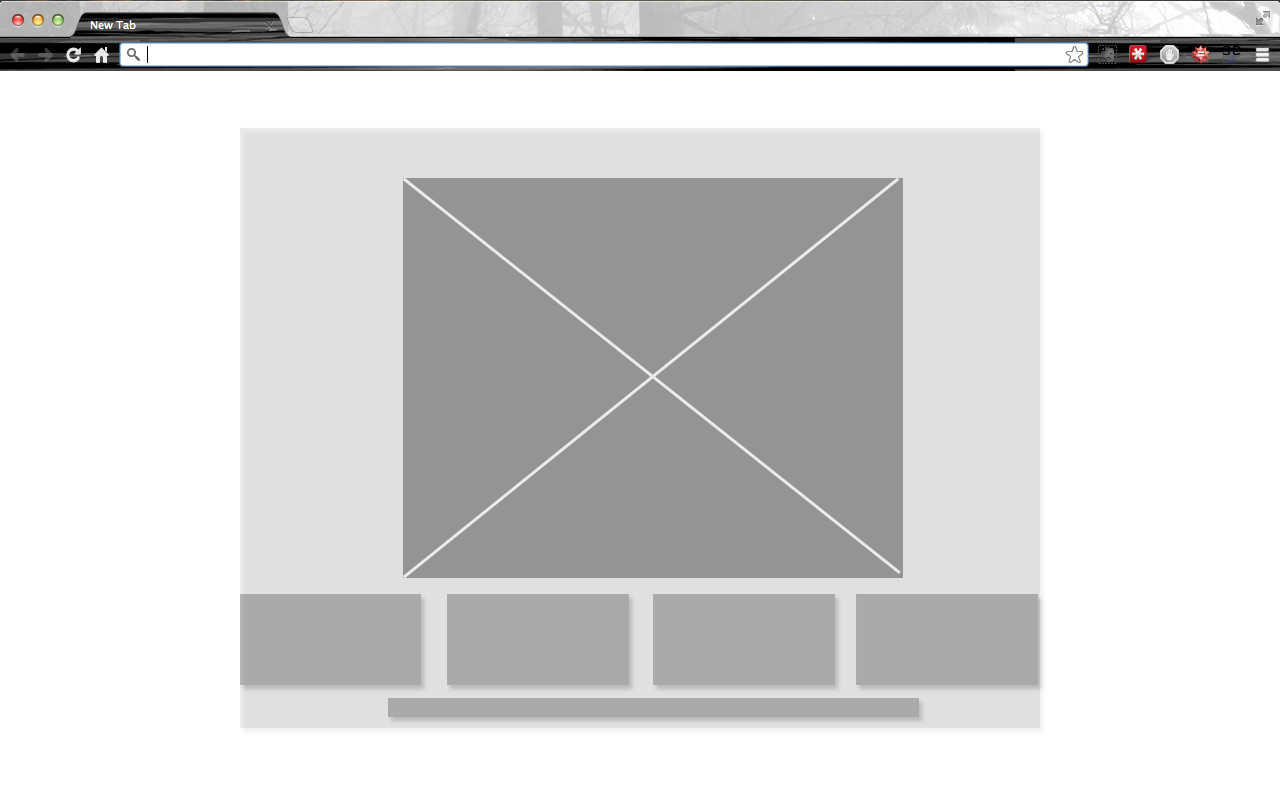
\includegraphics[width=0.5\textwidth]{1_IntroPage.jpg}
		\caption{Landing page wireframe diagram. }
		\label{fig:landingpagewireframe}
	\end{figure}
	
	These buttons will direct the user to different areas of the game space, and include Start (begin the game), Credits (display a lightbox of game credits), Rules (display a lightbox of gameplay rules), and Scores (send the player to a leaderboard page). There will also be provided, underneath the buttons, a link to the github repository containing the game project files. The layout of this landing page can be seen in 	Figure \ref{fig:landingpagewireframe}.
	
	\item[\textbf{Lightbox:}] \hspace{2em} Lightbox displays will be provided for the targets of the Credits and Rules buttons. These light-boxes will consist of a central section to provide the information relevant to the button choice, and an outer section to darken the background of the page and focus the user’s attention on the central content area. This design can be seen displayed in Figure \ref{fig:lightbox}. 
	
	\begin{figure}[h]
		\centering
		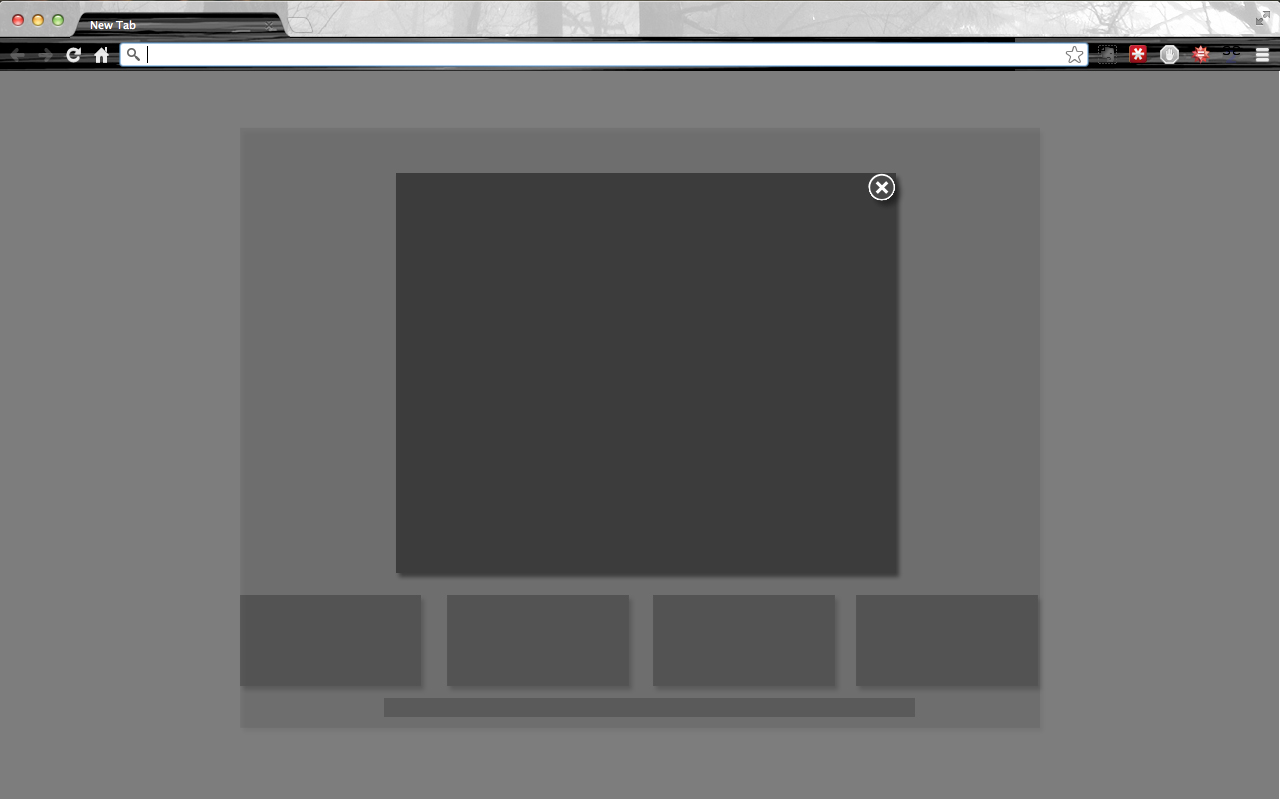
\includegraphics[width=0.5\textwidth]{2_rulesCreditsScoresLightbox.jpg}
		\caption{Lightbox diagram. }
		\label{fig:lightbox}
	\end{figure}
	
	\item[\textbf{Name and Age:}] \hspace{4em} The next view the user will be presented by upon clicked the Begin Game button is a form whose purpose is to gather the user’s name and age. This form can be seen in Figure \ref{fig:userinfo}.
	
	\begin{figure}[h]
		\centering
		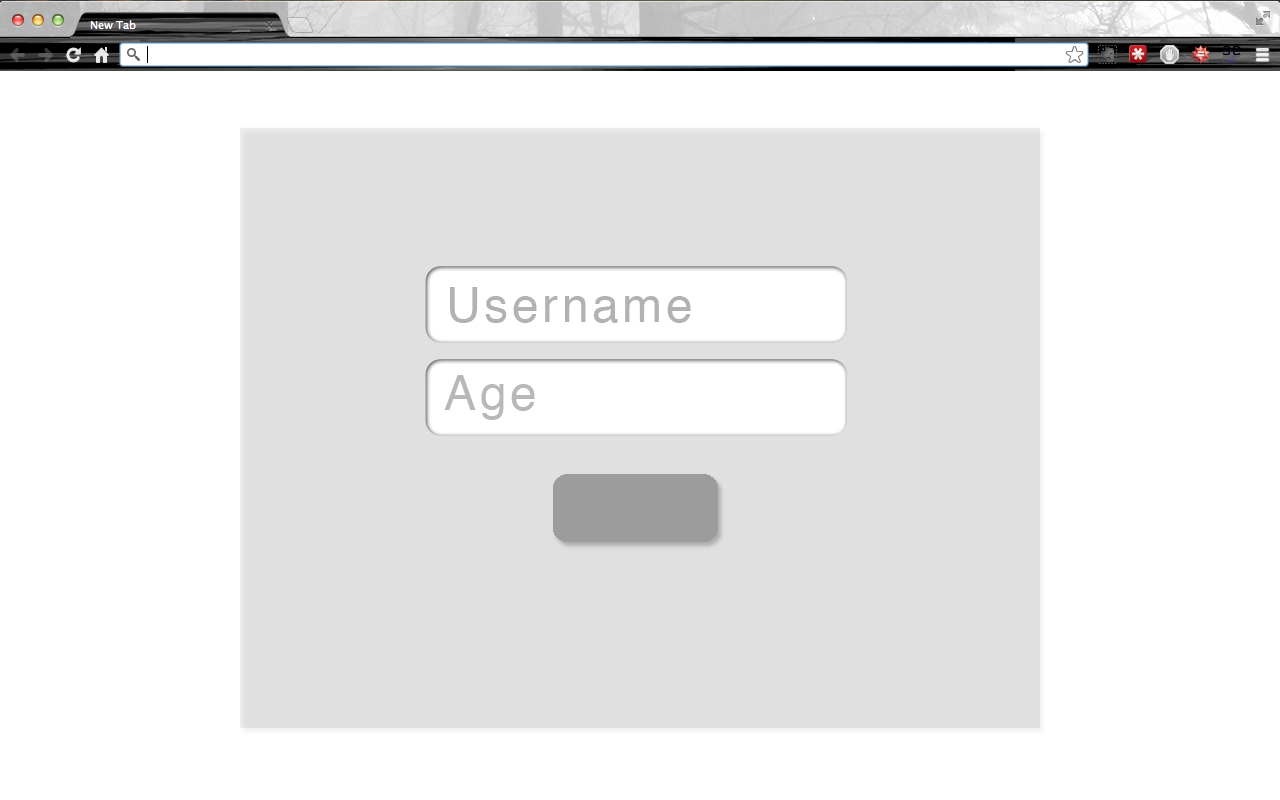
\includegraphics[width=0.5\textwidth]{3_UsernameAge.jpg}
		\caption{User information collection diagram. }
		\label{fig:userinfo}
	\end{figure}
	
	\item[\textbf{Choose Player:}] \hspace{4em} After entering the name and age information, the user is directed to the player choice page. In this page, the user selects one of 6 characters, 3 rats and 3 cats, to be their player avatar. A large central box displays the currently selected avatar, and a scrolling filmstrip of thumbnails sits below it allowing the user to choose the character avatar they desire. Below this filmstrip are two buttons, one to go back and one to go forward. Please see the appendix for a gallery of character and concept art. The Choose Player screen can be seen in Figure \ref{fig:chooseplayer}. 
	
	\begin{figure}[h]
		\centering
		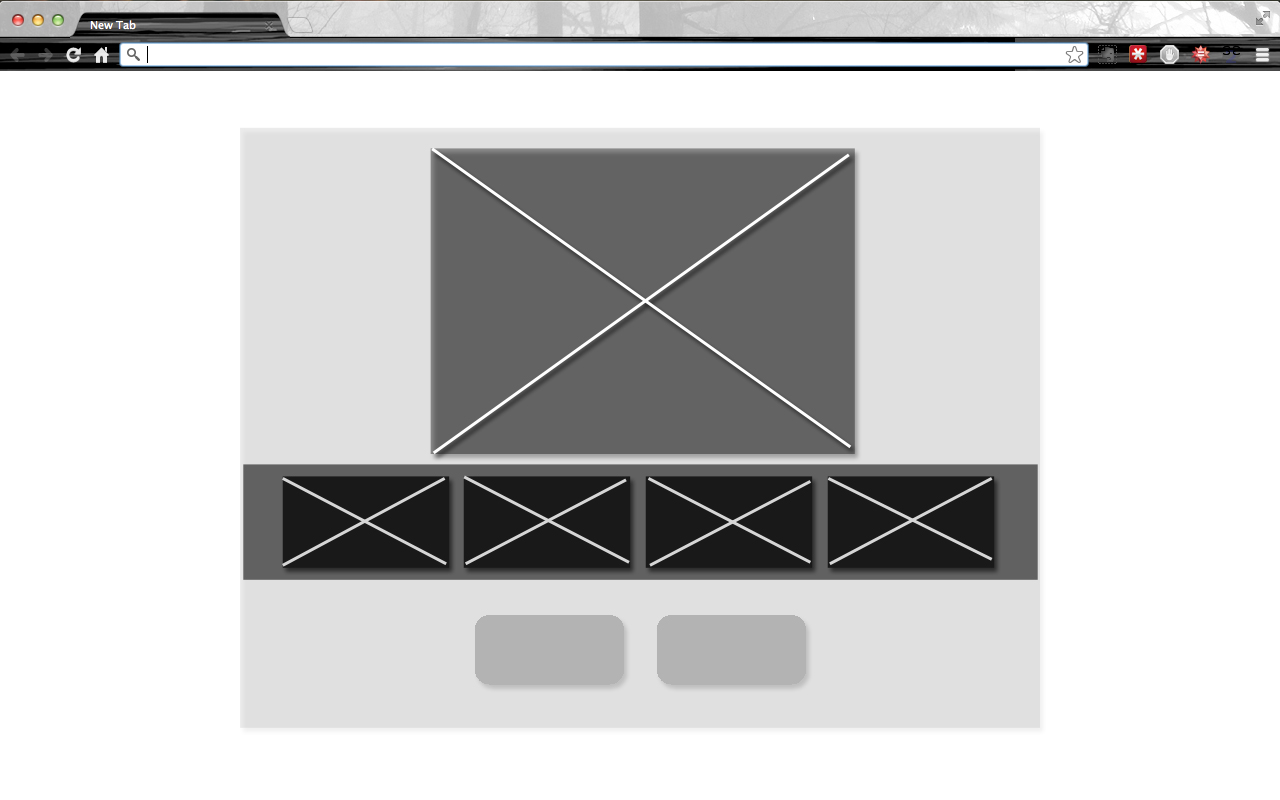
\includegraphics[width=0.5\textwidth]{4_ChoosePlayer.jpg}
		\caption{Player choice diagram. }
		\label{fig:chooseplayer}
	\end{figure}	
	
	\item[\textbf{Select Difficulty:}] \hspace{5em}The player is then directed to the difficulty selection interface. Like the previous interface, there is a large central box and scrolling filmstrip below it. Rather than player characters however, this filmstrip contains three difficulty settings; easy, medium and hard. The central box displays an image correlated with that difficulty level. There are buttons provided for forward and backwards navigation as well. This layout can be seen in Figure \ref{fig:difficulty}.
	
	\begin{figure}[h]
		\centering
		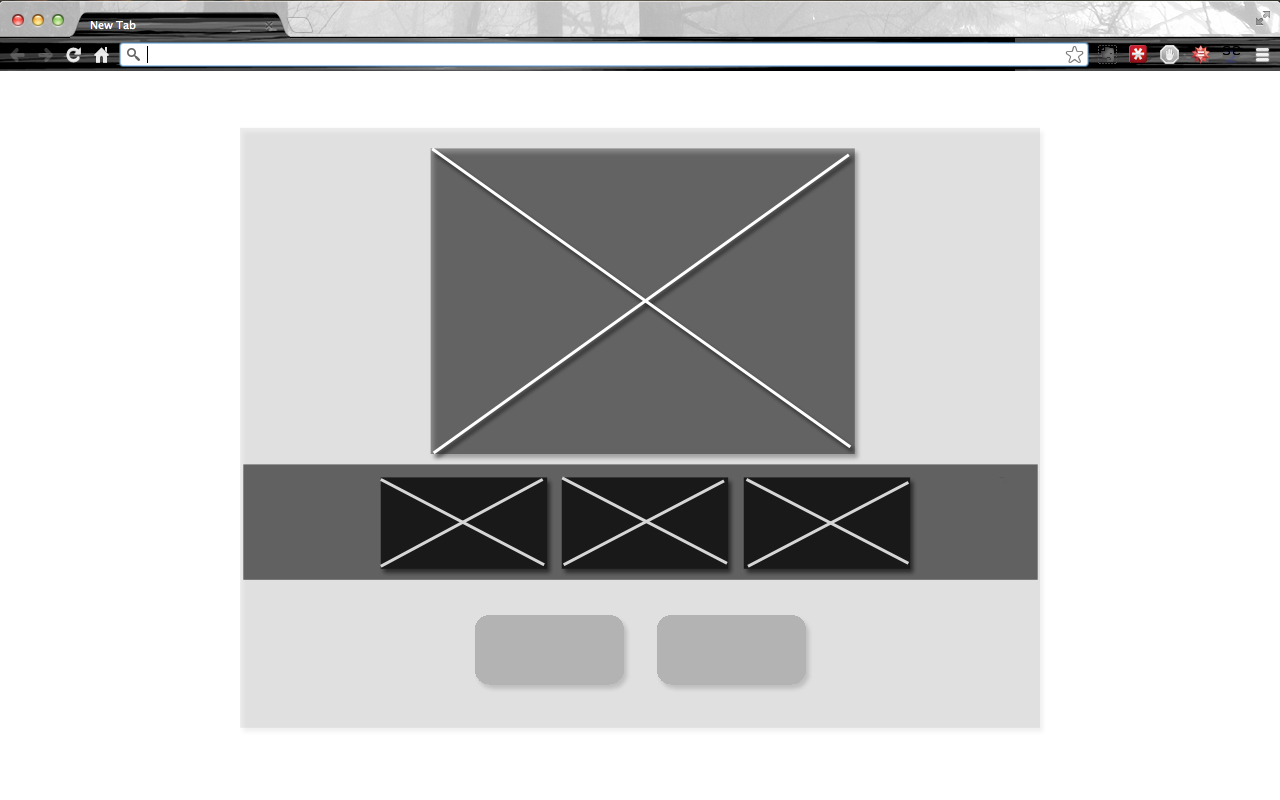
\includegraphics[width=0.5\textwidth]{5_ChooseDifficulty.jpg}
		\caption{Difficulty level diagram. }
		\label{fig:difficulty}
	\end{figure}
	
	\item[\textbf{Game Space:}] \hspace{4em} The final screen available to the player is the game space. This interface facilitates the player’s interaction with the actual flow of the game. There are several sections to this play space. There are two areas for the cards in play, the 4 cards on the top of the screen being for the opponent and the 4 on the bottom being for the player. The deck and discard piles are located between the two active card spreads, with the deck being on the right and the discard to its left. 
	
	In addition, there is a large area to the right of the interface which is used to display the active card (drawn from the discard or draw pile). A button below it is used by the player to “knock”, or end a round. This button will be active only on the player’s turn. In the upper left corner of the screen, there is a section for administrative utilities outside of the regular gameplay. This section includes the functionality to end the game, got back to the home screen or pull up the game rules (in a lightbox) at any time. After the game concludes, a lightbox containing the results is displayed to the user. This layout can be viewed in Figure \ref{fig:gamespace}.

	\begin{figure}[h]
		\centering
		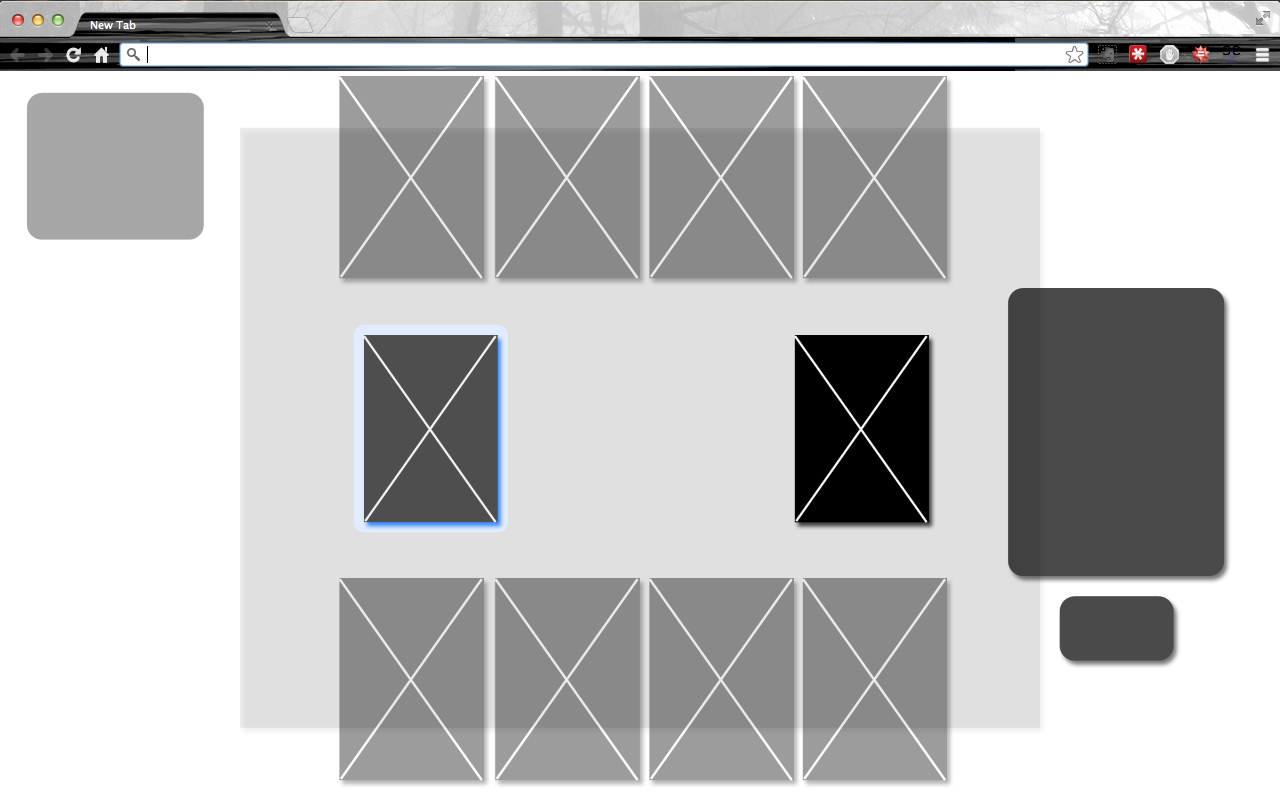
\includegraphics[width=0.5\textwidth]{6_GameSpace.jpg}
		\caption{Main game space diagram. }
		\label{fig:gamespace}
	\end{figure}

	\item[\textbf{Final Notes:}] \hspace{3em} In keeping with W3 statistics for modern screen size use, the interface will be designed to accommodate a viewport of 800x600 pixels. The interface should be flexible enough to scale with a reasonable degree of success to larger and smaller screen sizes. 
	
	The next actions of a player and their available options will be indicated by glowing areas of the gameboard. For example, when a player must decide between drawing from the Deck or from the Discard Pile, both of these objects will have a glowing effect applied to them to indicate potential choices. This glow can be seen surrounding the discard pile in Figure \ref{fig:gamespace}. 
	
	\end{description}

\subsection{Game Play}
\label{subsec:gameplay}

	\begin{figure}[h]
		\centering
		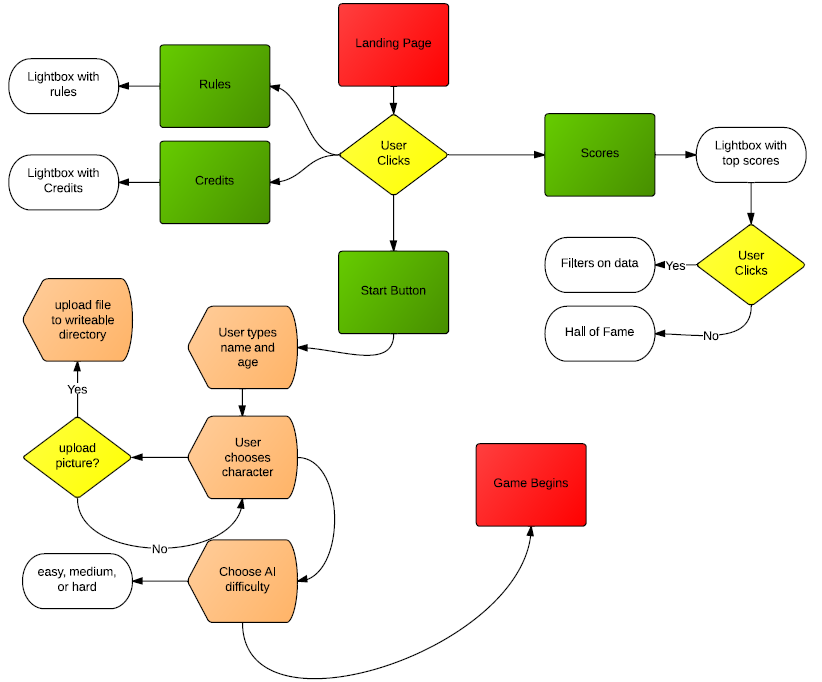
\includegraphics[width=0.5\textwidth]{landingpage.png}
		\caption{Landing page control flow diagram. }
		\label{fig:landingpage}
	\end{figure}

	The user is presented with the initial landing screen described in \S\ref{subsec:ui}, the execution flow is described in figure \ref{fig:landingpage}. The initial landing page is handled by the MainHandler controller and will use asynchronous post requests through jQuery to create light-boxes to display the Rules and Credits pages. The scores page shall exist on its own page due to its more complex nature and will allow players to see leader-boards and filter scoring information. Once A Player decides to start the game, their information will be gathered and an account created, the program will then divert control to the Game controller.

	\begin{figure}[h]
		\centering
		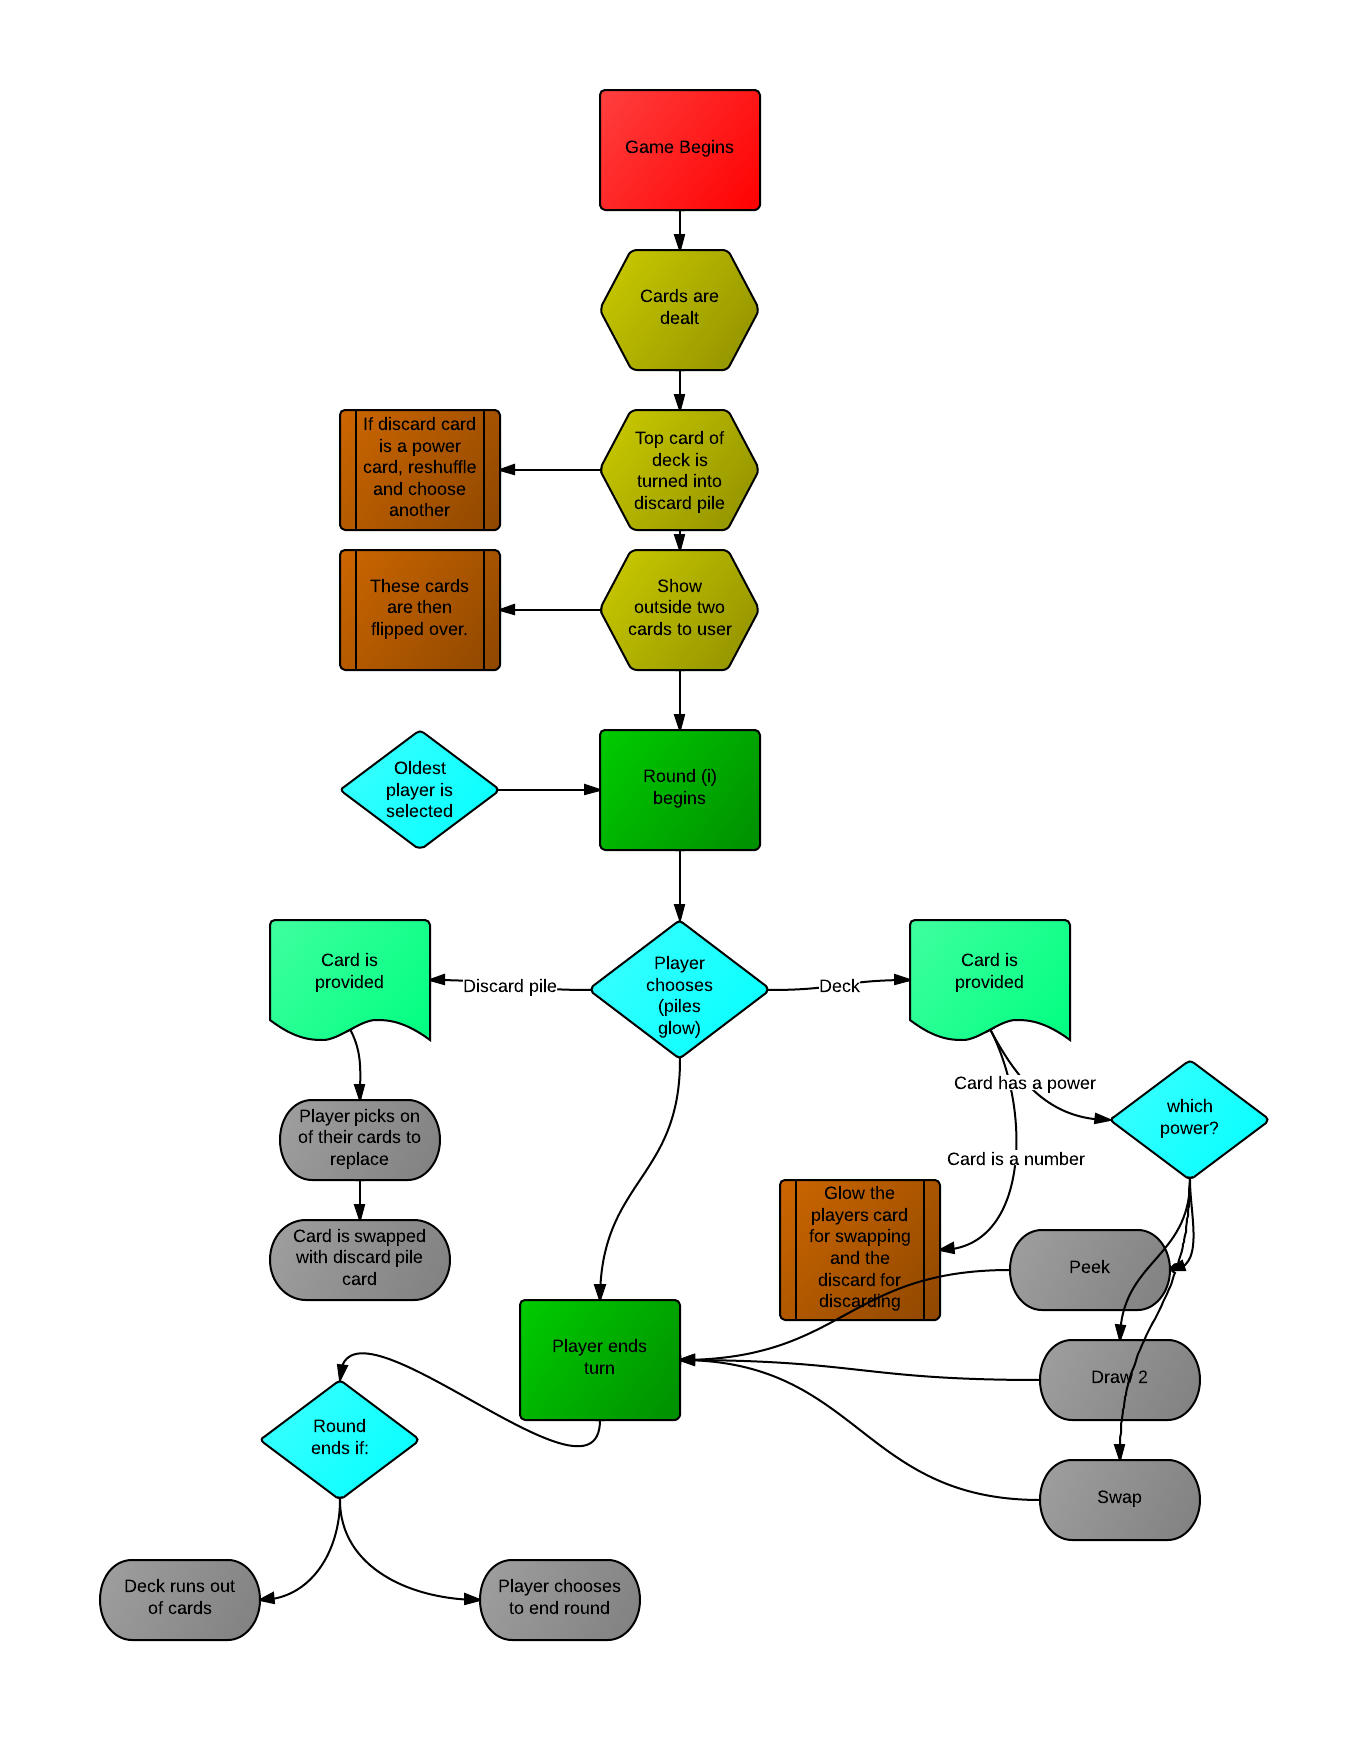
\includegraphics[width=0.5\textwidth]{gameplay.png}
		\caption{Game execution flow detailing initial setup and actions within a round. }
		\label{fig:gameplay}
	\end{figure}

	Once a user has begun the game the initial steps of dealing and selected a player to go first are executed. This requires no input from the user and consists primarily of animations and effects. Once a round begins, each player takes turns following the rules of the game specified in \S\ref{sec:rules}. 

	During a turn, a user is shown their possible actions to take by Glow-ing the cards and options available to them. At the beginning of the turn, the deck and discard piles are glown, indicating the User may select either to draw from the deck or discard pile. Note that in a sidebar, help text shall be displayed to indicate what the User should do if the visual queues are not enough information. Once a user has selected a card, they may choose to use it or to discard it. The use of each type of card is defined below and the sequence of actions defined for power cards displayed in figure \ref{fig:powact}.
	\begin{description}
		\item[Numeric] \hspace{1em} A numeric card may be swapped with any of the player's cards. The card is shown to the user, and their cards glown. Upon selection of a card, the selected card is discarded and replaced in the player's hand by the drawn card.
		\item[Peek] A peek card allows a user to look at a single card in their hand. If used, the player's cards glow and they are able to select the card to view.
		\item[Swap] A swap card allows a user to swap one of their cards with a card from the opponents hand. No cards are viewed. The player's cards are glown, allowing the player to select their card to switch. After selection, the opponents cards are glown and the player chooses the opponent card to swap with. 
		\item[Draw2] When a player draws a Draw 2 card they are allowed to draw up to 2 more cards from the deck or discard pile. The deck and discard piles glow indicating the need for a selection. Once a user draws a card, they may choose to use the card or to discard it. If a player uses a card, the draw 2 card is no longer in affect and after performing the actions allowed by the drawn card, their turn ends. 
	\end{description}
	
	\begin{figure}[h]
		\centering
		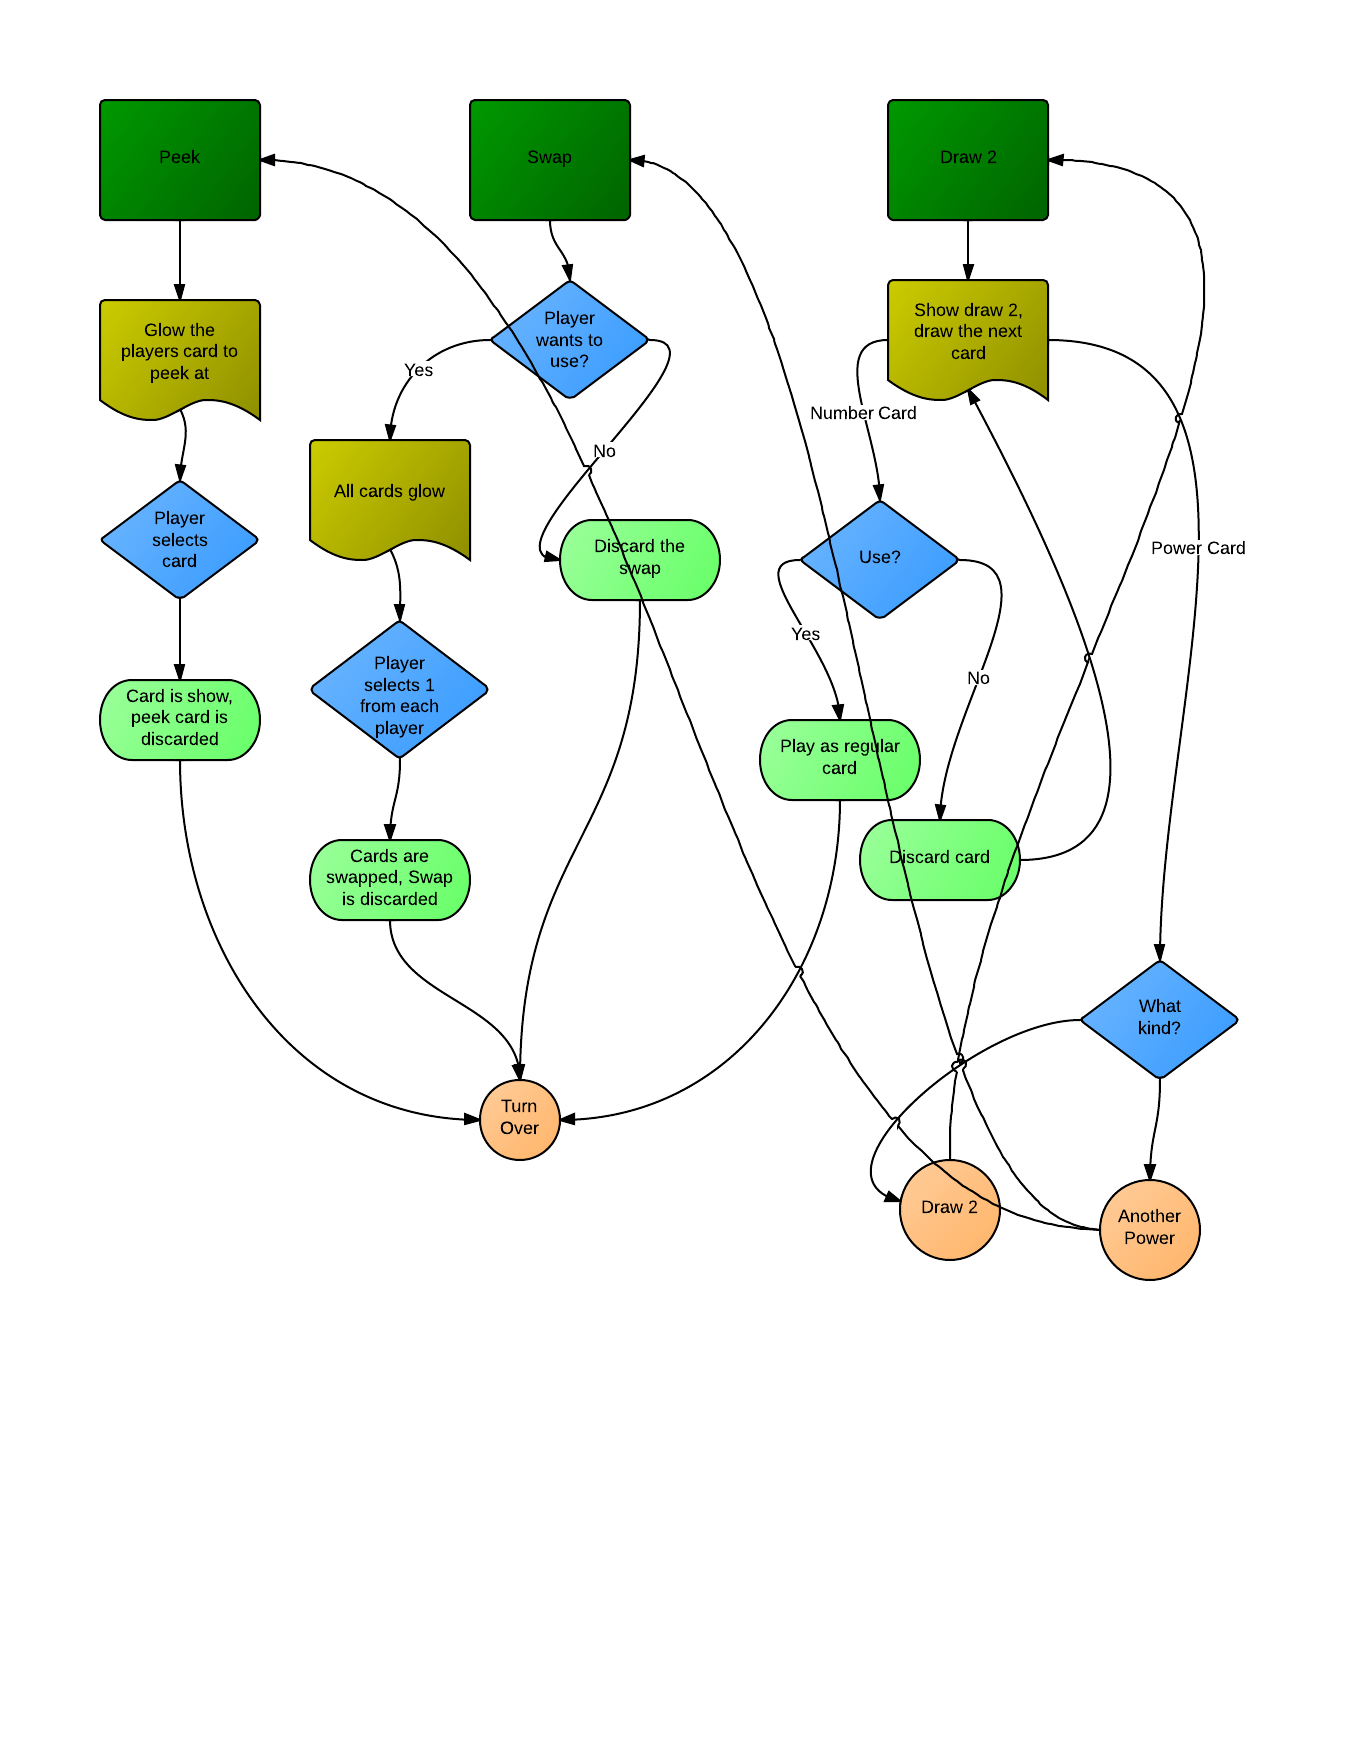
\includegraphics[width=0.5\textwidth]{powercardactions.png}
		\caption{Sequence of actions to be taken upon using any power card.}
		\label{fig:powact}
	\end{figure}

	When a round ends, the score is added to an overall score for the game, once a Player or AI reaches 60 or more points, the game ends. 

\subsection{The State Stack }
\label{subsec:urlhandstack}

	The execution of the program is driven through user interactions, in order to keep track of the game environment within a REST environment like an HTML document we create use a stack of possible states the System can be in. These states are defined as follows:
	\begin{itemize}
		\item \bfseries waitingForDraw \mdseries Iindicates the System shall glow the discard and deck cards, and await user  interaction.
		\item \bfseries waitingForPCard \mdseries Indicates the System shall glow the players cards and await user interaction.
		\item \bfseries HAL \mdseries The AI takes control of the game and processes its turn. 
		\item \bfseries playerChoice \mdseries A player has drawn any card from the deck and must choose to either discard or use it.
		\item \bfseries draw2PlayerChoice  \mdseries This is a special playerChoice state due to the nature of the draw 2 power card, the user is able to draw multiple cards and process each of those states while in this state.
	\end{itemize}

	The URL's handlers specified in \S\ref{subsec:arch} deal with actual pages defined within html. However there also exist a python Handler for each of the states. The following table indicates which states map to which controller:
	
	\begin{center}
		\begin{tabular}{| c | c |}\hline
			\multicolumn{1}{|c}{State} & \multicolumn{1}{c|}{ Handler Name }\\\hline
			\texttt{waitingForDraw} & waitingForDHandler\\\hline
			\texttt{waitingForPCard} & waitingForPCHandler\\\hline
			\texttt{HAL} & opponentAIHandler\\\hline
			\texttt{playerChoice} & playerChoiceHandler\\\hline
			\texttt{draw2PlayerChoice} & draw2ChoiceHandler\\\hline
		\end{tabular}
	\end{center}

\subsection{Character Design and Concept Art}
\label{subsec:cdesign}

\subsection{Timeline and Delivery}
\label{subsec:timeline}

	The following table describes the Work To Be Done (WTBD) during any individual week of the project. Delivery of WTBD will be reviewed during weekly team meetings. Code review and test cases will also take place during these meetings, and any expansion on scheduling for the project will be done as well. The project trajectory and timeline of deliverables is as follows:

	\begin{center}
		\begin{tabular}{ c |  p{0.35\textwidth} }
			Week of & Work to be done\\\hline
			&\\
			2/25 & HTML templates and css for Rules, Scores, landing page\\
			3/4 & Shell classes, Handlers, datastore\\
			3/11 & Model and view interfaces\\
			3/18 & Basic turn functionality\\
			3/25 &  Ability to play basic game (no power cards). Begin gathering test data\\
			4/1 & Incorporate power cards and gather more test data. Deliverable 2 due\\
			4/8 & Debugging and polishing game\\
			4/15 & Documentation creation. Group presentation preparation\\
			4/22 & Final due, Give presentation and finalize client product\\
		\end{tabular}
	\end{center}

\section{Summary}
\label{sec:summary}

	It is our desire that this implementation of the Rat-a-Tat-Cat card game capture the spirit and mechanics of the original game while adapting it to an interactive, web-driven and graphically pleasing format. This software implementation of Rat-a-Tat-Cat should be stable, robust, and eminently usable, providing players with an intuitive and consistently enjoyable gameplay experience in a natural interface. This specifications document is intended to provide the necessary framework to both implement and measure the success of these requirements, as well as set followable engineering standards to facilitate the creative process and satisfy the client’s inquiries and expectations.

\section{Appendix}
\label{sec:appendix}

\subsection{Rat Characters}
\label{subsec:ratcharacters}

	\begin{figure}[h]
		\centering
		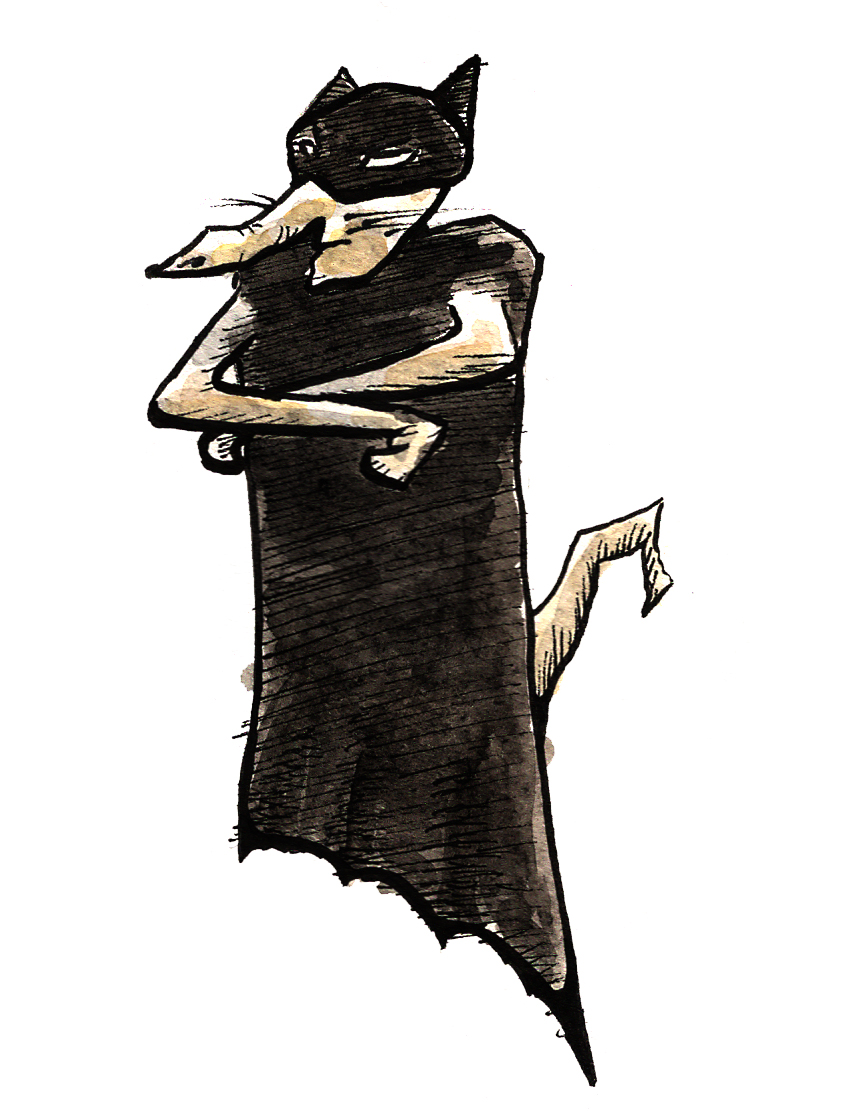
\includegraphics[width=0.5\textwidth]{Rat_Ratman.jpg}
		\caption{The character of "The Ratman".}
		\label{fig:ratman}
	\end{figure}

	\begin{figure}[h]
		\centering
		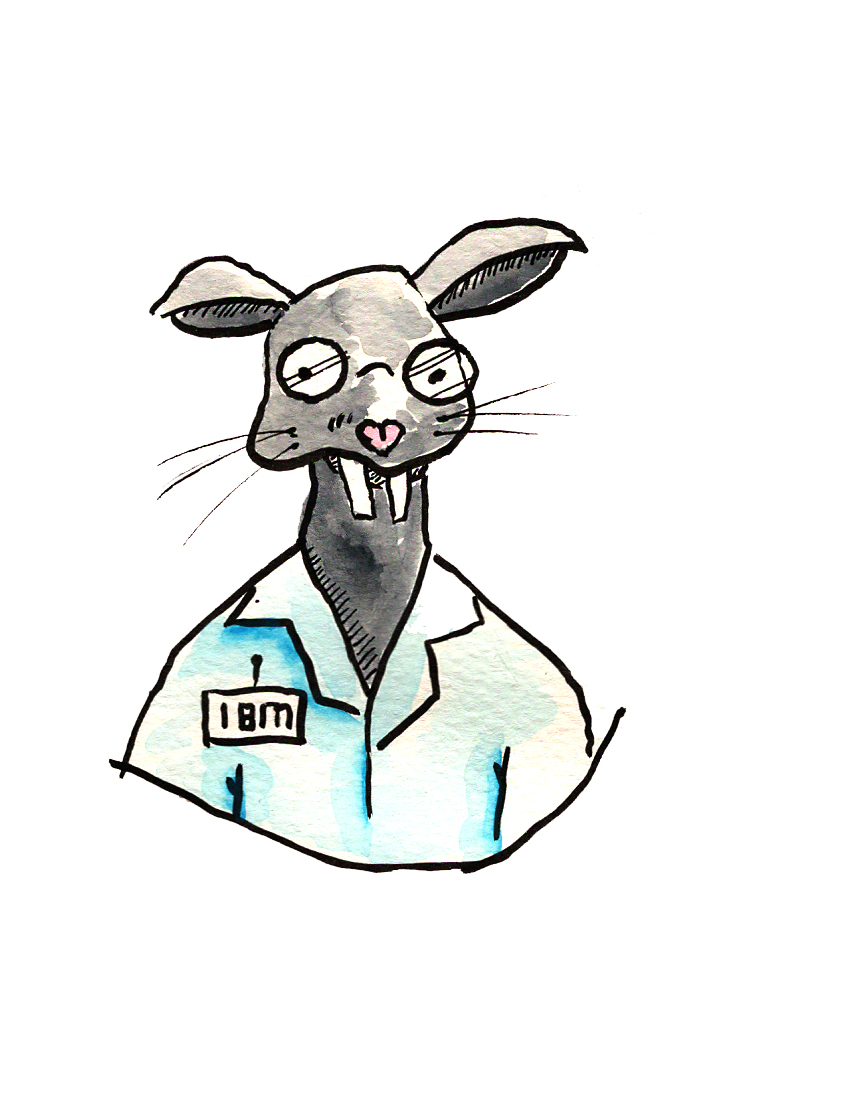
\includegraphics[width=0.5\textwidth]{Rat_Jason.jpg}
		\caption{The character of "Jason H.".}
		\label{fig:jason}
	\end{figure}
	
	\begin{figure}[h]
		\centering
		
\includegraphics[width=0.5\textwidth]{Rat_Betty.jpg}
		\caption{The character of "Betty, the Rat Queen".}
		\label{fig:betty}
	\end{figure}

\end{document}